\باب{سمتی میدان میں تکمل}\شناخت{باب_سمتی_میدان_میں_تکمل}
\موٹا{ایک جائزہ}\quad
اس باب  کا موضوع  سمتی میدان میں تکمل ہے۔ اس باب کی ریاضی کو برقناطیسیت  کے خواص   بیان کرنے کے لئے، تاروں میں حرارت  کے بہاو پر غور ، اور  مصنوعی سیارہ کو  مدار میں منتقل کرنے  کے لئے درکار توانائی کے حصول کے لئے استعمال کیا جاتا ہے۔

\حصہ{لکیری تکمل}
جب فضا میں  تفاعل \عددی{f(x,y,z)} کے دائرہ کار سے منحنی \عددی{\kvec{r}(t)=g(t)\ai+h(t)\aj+k(t)\ak,\,a\le t\le b}  گزرے تب اس   منحنی  کے ساتھ چلتے ہوئے \عددی{f}  کی قیمتیں مرکب تفاعل \عددی{f(g(t),h(t),k(t))} دیگا۔ نقطہ \عددی{a} سے \عددی{b} تک لمبائی قوس  کے لحاظ سے اس مرکب تفاعل کے تکمل کو قوس کے ساتھ \عددی{f} کا  \اصطلاح{لکیری  تکمل}\فرہنگ{تکمل!لکیری}\حاشیہب{line integral}\فرہنگ{integral!line} کہتے ہیں۔  تین بعدی جیومیٹری کے باوجود،  لکیری تکمل حقیقی اعداد کے وقفہ پر حقیقی قیمت تفاعل کا سادہ تفاعل ہو گا۔

لکیری تکمل کی اہمیت اس کے استعمال میں ہے۔ ان تکملات  کی مدد سے ہم  متغیر قوتوں کی فضا میں راہ پر کام    اور قوس  کے ساتھ یا  سرحد پار کرتی سیال کی شرح بہاو  کا حساب کرتے ہیں۔

\begin{figure}
\centering
\begin{tikzpicture}[font=\small,declare function={fx(\x)=sin(\x)+1/3*cos(3*\x);fy(\t)=cos(\t);fz(\t)=\t/100;}]
\coordinate (O) at (-0.5,-1);
\draw[smooth, domain=5:120]plot ({\x/30},{fx(\x)});
\foreach \t in {1,3.2,4.6,7,9,11}{\path[| mark=0.5] ({(\t-0.1)/3},{fx((\t-0.1)*10)}) -- ({(\t+0.1)/3},{fx((\t+0.1)*10)});}
\draw[] ({7.5/3},{fx(7.5*10)})node[circ]{}node[right,yshift=-1ex]{$(x_k,y_k,z_k)$};
\draw[-stealth](O)--++(-0.5,-0.5)node[left]{$x$};
\draw[-stealth](O)--++(3,0)node[right]{$y$};
\draw[-stealth](O)--++(0,2)node[left]{$z$};
\draw[-latex](O)--({4/3},{fx(4*10)})node[pos=0.5,below]{$\kvec{r}$};
\draw[] ({1/3},{fx(1*10)})node[xshift=-2ex,yshift=2ex]{$t=a$};
\draw[] ({11/3},{fx(11*10)})node[xshift=2ex,yshift=2ex]{$t=b$};
\draw[decorate,decoration={brace,amplitude=5pt, raise=5pt}] ({7/3},{fx(7*10)})--({9/3},{fx(9*10)})node[above left,shift={(145:5pt)}]{$\Delta s_k$};
\end{tikzpicture}
\caption{
منحنی \عددی{\kvec{r}=g(t)\ai+h(t)\aj+k(t)\ak} کو \عددی{t=a} اور \عددی{t=b} کے بیچ قوسچوں میں تقسیم کیا گیا ہے۔ ایک علامتی  قوسچہ کی لمبائی \عددی{\Delta s_k} ہے۔
}
\label{شکل_کثیر_قوسچہ}
\end{figure}

\جزوحصہء{تعریفات اور  علامتیت}
فرض کریں تفاعل \عددی{f(x,y,z)}  کے  دائرہ کار میں منحنی \عددی{\kvec{r}(t)=g(t)\ai+h(t)\aj+k(t)\ak,\,a\le t\le b} پائی جاتی ہے۔ ہم اس منحنی کی،  متناہی تعداد کی  قوسچوں میں، خانہ بندی کرتے ہیں (شکل \حوالہ{شکل_کثیر_قوسچہ})۔ ایک علامتی قوسچہ کی لمبائی \عددی{\Delta s_k} ہو گی۔ ہم ہر قوسچہ پر  ایک نقطہ \عددی{(x_k,y_k,z_k)}  منتخب کر کے درج ذیل مجموعہ لیتے ہیں۔
\begin{align}\label{مساوات_میدان_خطی_تکمل_الف}
J_n=\sum\limits_{k=1}^{n} f(x_k,y_k,z_k)\Delta s_k
\end{align}
اگر \عددی{f} استمراری ہو اور \عددی{g}، \عددی{h}،  اور \عددی{k} کے  اول تفرقات استمراری ہوں تب جیسے جیسے  \عددی{n} بڑھایا جائے، \عددی{\Delta s_k}  صفر تک پہنچے گی اور   مساوات \حوالہ{مساوات_میدان_خطی_تکمل_الف} کا مجموعہ  ایک حد کو پہنچے گا۔ ہم اس حد کو \اصطلاح{ \عددی{a} تا \عددی{b} اس قوس پر \عددی{f} کا تکمل} کہتے ہیں۔  قوس کو \عددی{C} سے ظاہر کرتے ہوئے  اس تکمل کو علامتی طور پر درج ذیل لکھا جاتا ہے۔
\begin{align}\label{مساوات_میدان_خطی_تکمل_ب}
\int_C f(x,y,z)\dif s\quad \quad \text{\RL{"\عددی{C} پر \عددی{f} کا تکمل"}}
\end{align}

\جزوحصہء{ہموار منحنیات پر تکمل کی قیمت کا حصول}
اگر وقفہ \عددی{a\le t\le b} پر \عددی{\kvec{r}(t)} ہموار ہو   (\عددی{\kvec{v}=\tfrac{\dif\kvec{r}}{\dif t}}   استمراری  ہو اور کبھی بھی \عددی{\kvec{0}} نہ ہو)   تب ہم \عددی{\dif s}  کو بیان کرنے کے لئے درج ذیل مساوات استعمال کر سکتے ہیں  چونکہ  اس سے \عددی{\dif s=\abs{\kvec{v}(\tau)}\dif t} لکھا جا سکتا ہے۔
\begin{align*}
s(t)=\int_a^t \abs{\kvec{v}(\tau)} \dif \tau\quad\text{\small\RL{حصہ \حوالہ{حصہ_سمتی_تفاعل_لمبائی_قوس_اور_اکائی_سمتیہ} کی  مساوات \حوالہ{مساوات_سمتی_تفاعل_لمبائی_قوس_ت} میں \عددی{t_0=a}}}
\end{align*}
اعلٰی احصاء کا ایک مسئلہ کہتا ہے کہ ایسی صورت میں ہم  درج ذیل طریقہ سے \عددی{C} پر \عددی{f} کے تکمل کی قیمت حاصل کر  سکتے ہیں۔
\begin{align*}
\int_C f(x,y,z)\dif s=\int_a^b f(g(t),h(t),k(t))\abs{\kvec{v}(t)}\dif t
\end{align*} 
ہم جس مقدار معلوم روپ کو بھی استعمال کریں، جب تک زیر استعمال مقدار معلوم   روپ ہموار ہو، یہ کلیہ ہمیں تکمل کی قیمت دیگا۔ 

\جزوحصہء{لکیری تکمل کی قیمت کا حصول}
منحنی  \عددی{C} پر استمراری تفاعل \عددی{f} کا  تکمل لینے کے لئے
\begin{enumerate}[a.]
\item
\عددی{C} کی مقدار معلوم روپ تلاش کریں:
\[\kvec{r}(t)=g(t)\ai+h(t)\aj+k(t)\ak,\quad a\le t\le b\]
\item
درج ذیل تکمل کی قیمت حاصل کریں۔
\begin{align}\label{مساوات_میدان_خطی_تکمل_پ}
\int_Cf(x,y,z)\dif s=\int_a^bf(g(t),h(t),k(t))\abs{\kvec{v}(t)}\dif t
\end{align}
\end{enumerate}

دھیان رہے کہ مستقل تفاعل \عددی{f=1} کی صورت میں مذکورہ بالا تکمل \عددی{C} کی لمبائی دیگا۔

%====================
\ابتدا{مثال}\شناخت{مثال_میدان_راہ_الف}
مبدا سے  نقطہ \عددی{(1,1,1)} تک قطع پر \عددی{f(x,y,z)=x-3y^2+z} تکمل کریں (شکل \حوالہ{شکل_مثال_میدان_راہ_الف})۔

حل:\quad
ہم  ذہن میں آنے والا سادہ ترین مقدار معلوم روپ استعمال کرتے ہیں
\[\kvec{r}(t)=t\ai+t\aj+t\ak,\quad 0\le t\le 1\]
جس کی اجزاء کے اول تفرقات استمراری ہیں اور \عددی{\abs{\kvec{v}(t)}=\sqrt{1^2+1^2+1^2}=\sqrt{3}} کبھی بھی \عددی{\kvec{0}} نہیں ہو سکتا ہے لہٰذا  یہ مقدار معلوم روپ ہموار ہے۔ یوں   \عددی{C} پر \عددی{f} کا تکمل درج ذیل ہو گا۔
\begin{align*}
\int_C f(x,y,z)\dif s&=\int_0^1 f(t,t,t)(\sqrt{3})\dif t&&\text{\RL{مساوات \حوالہ{مساوات_میدان_خطی_تکمل_پ}}}\\
&=\int_0^1 (t-3t^2+t)\sqrt{3}\dif t\\
&=\sqrt{3}\int_0^1 (2t-3t^2)\dif t=\sqrt{3}\big[t^2-t^3\big]_0^1=0
\end{align*} 
\انتہا{مثال}
%===================
\begin{figure}
\centering
\begin{minipage}{0.45\textwidth}
\centering
\begin{tikzpicture}[]
\begin{axis}[clip=false,view/h=110,small,axis lines=middle,xtick={\empty},ytick={\empty},ztick={\empty},enlargelimits=true, xlabel={$x$}, ylabel={$y$},zlabel={$z$}, xlabel style={anchor=north},ylabel style={anchor=west},zlabel style={anchor=south},colormap={}{gray(0cm)=(0.6);gray(1cm)=(0.9);}]
\addplot3[]plot coordinates {(0,0,0)(1,1,1)}node[pos=1,circ]{}node[pos=1,right]{$(1,1,1)$}node[pos=0.5,above]{$C$};
\addplot3[dashed]plot coordinates {(1,1,1)(1,1,0)(0,0,0)};
\addplot3[]plot coordinates {(1,1,0)}node[right]{$(1,1,0)$};
\end{axis}
\end{tikzpicture}
\caption{تکمل کی راہ (مثال \حوالہ{مثال_میدان_راہ_الف})۔}
\label{شکل_مثال_میدان_راہ_الف}
\end{minipage}\hfill
\begin{minipage}{0.45\textwidth}
\centering
\begin{tikzpicture}[]
\begin{axis}[clip=false,view/h=110,small,axis lines=middle,xtick={\empty},ytick={\empty},ztick={\empty},enlargelimits=true, xlabel={$x$}, ylabel={$y$},zlabel={$z$}, xlabel style={anchor=north},ylabel style={anchor=west},zlabel style={anchor=south},colormap={}{gray(0cm)=(0.6);gray(1cm)=(0.9);},zmax=0.75]
\addplot3[]plot coordinates {(0,0,0)(1,1,0)}node[pos=0,circ]{}node[pos=0,pin=135:{$(0,0,0)$}]{}node[pos=1,circ]{}node[pos=1,right]{$(1,1,0)$}node[pos=0.5,below]{$C_1$};
\addplot3[]plot coordinates {(1,1,0)(1,1,1)}node[pos=1,circ]{}node[pos=1,right]{$(1,1,1)$}node[pos=0.75,right]{$C_2$};
\end{axis}
\end{tikzpicture}
\caption{تکمل کی راہ (مثال \حوالہ{مثال_میدان_راہ_ب})۔}
\label{شکل_مثال_میدان_راہ_ب}
\end{minipage}
\end{figure}


\جزوحصہ{جمع پذیری}
  اگر متناہی تعداد کی منحنیات \عددی{C_1}، \عددی{C_2}، \نقطے، \عددی{C_n} کو ایک دوسرے کے ساتھ جوڑ کر منحنی \عددی{C} حاصل کی جائے تب  \عددی{C} پر تفاعل کا تکمل ان منحنیات پر تفاعل کے تکملات کا مجموعہ ہو گا:
\begin{align}\label{مساوات_میدان_خطی_تکمل_ت}
\int_C f\dif s=\int_{C_1} f\dif s+\int_{C_2} f\dif s+\cdots+\int_{C_n} f\dif s
\end{align}

\ابتدا{مثال}\شناخت{مثال_میدان_راہ_ب}
مبدا سے نقطہ \عددی{(1,1,1)} تک  راہ \عددی{C_1} اور \عددی{C_2}  پر چل کر پہنچا جاتا ہے (شکل \حوالہ{شکل_مثال_میدان_راہ_ب})۔ یوں \عددی{C} ان کا اشتراک \عددی{C_1\cup C_2} ہو گا۔ تفاعل \عددی{f(x,y,z)=x-3y^2+z}  کے تکمل کی قیمت  \عددی{C_1\cup C_2} پر  تلاش کریں۔

حل:\quad
ہم \عددی{C_1} اور \عددی{C_2} کے لئے،  ذہن میں آنے  والے  سادہ ترین،  مقدار معلوم روپ  استعمال کرتے ہیں:
\begin{align*}
C_1:\quad \kvec{r}(t)&=t\ai+t\aj,\, 0\le t\le 1;\, \abs{\kvec{v}}=\sqrt{1^2+1^2}=\sqrt{2}\\
C_2:\quad \kvec{r}(t)&=\ai+\aj+t\ak,\, 0\le t\le 1;\, \abs{\kvec{v}}=\sqrt{0^2+0^2+1^2}=1
\end{align*}
ان مقدار معلوم روپ کے ساتھ درج ذیل حاصل ہو گا۔
\begin{align*}
\int_{C_1\cup C_2}f(x,y,z)\dif s&=\int_{C_1}f(x,y,z)\dif s+\int_{C_2}f(x,y,z)\dif s&&\text{\RL{مساوات \حوالہ{مساوات_میدان_خطی_تکمل_ت}}}\\
&=\int_0^1 f(t,t,0)\sqrt{2} \dif t+\int_0^1 f(1,1,t)(1)\dif t\\
&=\int_0^1 (t-3t^2+0)\sqrt{2}\dif t+\int_0^1(1-3+t)(1)\dif t\\
&=\sqrt{2}\big[\frac{t^2}{2}-t^3\big]_0^1+\big[\frac{t^2}{2}-2t\big]_0^1=-\frac{\sqrt{2}}{2}-\frac{3}{2}
\end{align*}
\انتہا{مثال}
%=======================

یہاں   مثال \حوالہ{مثال_میدان_راہ_الف} اور مثال \حوالہ{مثال_میدان_راہ_ب} کے نتائج پر غور کرتے ہیں۔اول، دیکھیں کہ  موزوں منحنی کے اجزاء \عددی{f} میں پر کرتے ہی  \عددی{t} کے لحاظ سے ایک  سادہ تکمل حاصل ہوتا ہے۔ دوم،  \عددی{C_1\cup C_2} پر \عددی{f} کا تکمل لینے کے لئے \عددی{C_1} اور \عددی{C_2} پر \عددی{f} کے علیحدہ علیحدہ تکملات لے کر نتائج  کا مجموعہ لیا جاتا ہے۔سوم،      مثال \حوالہ{مثال_میدان_راہ_الف} میں \عددی{C}  اور مثال \حوالہ{مثال_میدان_راہ_ب} میں \عددی{C_1\cup C_2} پر تکمل کے نتائج ایک دوسرے سے مختلف تھے۔ عموماً تفاعل کے لئے دو نقطوں کے بیچ مختلف راہ پر تکملات کے نتائج ایک دوسرے سے مختلف ہوں گے۔ البتہ بعض تفاعل کے لئے تکمل کی قیمت پر راہ کا کوئی اثر نہیں ہوتا ہے۔

\جزوحصہء{کمیت اور معیار اثر کا حساب}
ہم اسپرنگ اور تار کو فضا میں ہموار منحنی پر  استمراری کمیتی کثافت \عددی{\delta(x,y,z)} کی تقسیم تصور کرتے ہیں۔ یوں اسپرنگ یا تار کی کمیت، مرکز کمیت، اور ان کے معیار اثر اور  رداس دوار کا حساب    درج ذیل  کلیات سے کیا جائے گا۔ یہی کلیات باریک (پتلی) تار کے لئے بھی کارآمد ہوں گے۔
\begin{description}
\item{کیمت:}\quad
\(M=\iiint\limits_D \delta(x,y,z) \dif H\)
\item{محددی مستویات کے لحاظ سے اول معیار اثر:}
\[M_{yz}=\int_C x\delta \dif s,\quad M_{xz}=\int_C y\delta \dif s,\quad M_{xy}=\int_Cz\delta \dif s\]
\item{مرکز کمیت کے محدد:}
\[\bar{x}=\frac{M_{yz}}{M},\quad \bar{y}=\frac{M_{xz}}{M},\quad \bar{z}=\frac{M_{xy}}{M}\]
\item{معیار اثر:}
\begin{align*}
I_x&=\int_C(y^2+z^2)\delta \dif s & I_y&=\int_C(x^2+z^2)\delta \dif s\\
I_z&=\int_C(x^2+y^2)\delta \dif s& I_L&=\int_C r^2\delta \dif s
\end{align*}
جہاں  لکیر \عددی{L} سے نقطہ \عددی{(x,y,z)} تک فاصلہ \عددی{r(x,y,z)} ہے۔
\item{لکیر \عددی{L} کے لحاظ سے رداس دور:}\quad
\(R_L=\sqrt{\frac{I_L}{M}}\)
\end{description}

%==================================
\ابتدا{مثال}\شناخت{مثال_سمتی_تکمل_اسپرنگ}
ایک اسپرنگ درج ذیل پیچدار منحنی کے ساتھ ساتھ پایا جاتا ہے (شکل \حوالہ{شکل_مثال_سمتی_تکمل_اسپرنگ})۔
\[\kvec{r}(t)=(\cos t)\ai+(\sin t)\aj+t\,\ak,\quad 0\le t\le 2\pi\]
اس اسپرنگ کی کثافت مستقل تفاعل \عددی{\delta=1} ہے۔ اس اسپرنگ کی کمیت اور مرکز کمیت  اور محور \عددی{z} کے لحاظ سے   جمودی معیار اثر اور رداس دوار معلوم کریں۔

حل:\quad
ہم اسپرنگ کا خاکہ بناتے ہیں۔ تشاکلی کی بنا اس کا مرکز کمیت محور \عددی{z} پر  نقطہ \عددی{(0,0,\pi)} پر پایا جائے گا۔  باقی حساب کے لئے ہم \عددی{\abs{\kvec{v}(t)}} تلاش کرتے ہیں:
\begin{align*}
\abs{\kvec{v}(t)}&=\sqrt{\big(\frac{\dif x}{\dif t}\big)^2+\big(\frac{\dif y}{\dif t}\big)^2+\big(\frac{\dif z}{\dif t}\big)^2}\\
&=\sqrt{(-4\sin 4t)^2+(4\cos 4t)^2+1}=\sqrt{17}
\end{align*}
اب مذکورہ بالا کلیات استعمال کرتے ہوئے درج ذیل حاصل ہو گا۔
\begin{align*}
M&=\int\limits_{\text{پیچدار}} \delta \dif s=\int_0^{2\pi} (1)\sqrt{17}\dif t=2\pi\sqrt{17}\\
I_z&=\int\limits_{\text{پیچدار}} (x^2+y^2)\delta \dif s=\int_0^{2\pi}(\cos^2 4t+\sin^2 4t)(1)(\sqrt{17})\dif t\\
&=\int_0^{2\pi}\sqrt{17}\dif t=2\pi\sqrt{17}\\
R_z&=\sqrt{\frac{I_z}{M}}=\sqrt{\frac{2\pi\sqrt{17}}{2\pi\sqrt{17}}}=1
\end{align*}
دھیان رہے کہ محور \عددی{z} کے لحاظ سے رداس دوار عین اس بیلن کے رداس  جتنا ہے جس پر اسپرنگ لپیٹا گیا ہے۔
\انتہا{مثال}
%=====================

\begin{figure}
\centering
\begin{minipage}{0.45\textwidth}
\centering
\begin{tikzpicture}[declare function={fx(\t)=cos(deg(4*\t));fy(\t)=sin(deg(4*\t));fz(\z)=\t;}]
\begin{axis}[clip=false,view/h=110,small,axis lines=middle,xtick={1},ytick={\empty},ztick={pi,2*pi},zticklabels={$\pi$,$2\pi$},enlargelimits=true, xlabel={$x$}, ylabel={$y$},zlabel={$z$}, xlabel style={anchor=east},ylabel style={anchor=west},zlabel style={anchor=west},colormap={}{gray(0cm)=(0.6);gray(1cm)=(0.9);}]
\addplot3[domain=0:2*pi,variable=\t,samples y=0,samples=100]({fx(t)},{fy(t)},{fz(t)});
\addplot3[]plot coordinates {(0,0,pi)}node[circ]{};
\end{axis}
\end{tikzpicture}
\caption{اسپرنگ برائے مثال \حوالہ{مثال_سمتی_تکمل_اسپرنگ}}
\label{شکل_مثال_سمتی_تکمل_اسپرنگ}
\end{minipage}\hfill
\begin{minipage}{0.45\textwidth}
\centering
\begin{tikzpicture}[declare function={fy(\t)=cos(deg(\t));fz(\t)=sin(deg(\t));}]
\begin{axis}[clip=false,view/h=110,small,axis lines=middle,xtick={\empty},ytick={-1,1},ztick={0.57,1},zticklabels={$0.57$,$1$},enlargelimits=true, xlabel={$x$}, ylabel={$y$},zlabel={$z$}, xlabel style={anchor=east},ylabel style={anchor=west},zlabel style={anchor=south},colormap={}{gray(0cm)=(0.6);gray(1cm)=(0.9);},]
\addplot3[domain=0:pi,variable=\t,samples y=0,smooth]({0},{fy(t)},{fz(t)});
\addplot3[]plot coordinates {(0.1,0,0)}node[right,xshift=2ex]{$y^2+z^2=1,\, z\ge 0$};
\addplot3[]plot coordinates {(0,0,0.57)}node[circ]{};
\end{axis}
\end{tikzpicture}
\caption{محراب کا مرکز کمیت (مثال \حوالہ{مثال_سمتی_تکمل_قوس_کی_کمیت})۔}
\label{شکل_مثال_سمتی_تکمل_قوس_کی_کمیت}
\end{minipage}
\end{figure}
\ابتدا{مثال}\شناخت{مثال_سمتی_تکمل_قوس_کی_کمیت}
مستوی \عددی{yz} میں نصف دائرہ \عددی{y^2+z^2=1,\, z\ge 0} پر ایک  دبلا پتلا محراب پایا جاتا ہے (شکل \حوالہ{شکل_مثال_سمتی_تکمل_قوس_کی_کمیت})۔ محراب کے نقطہ \عددی{(x,y,z)} پر کثافت \عددی{\delta(x,y,z)=2-z} ہے۔ محراب کا مرکز کمیت تلاش کریں۔

حل:\quad
چونکہ یہ  محراب مستوی \عددی{yz} میں پایا جاتا ہے  اور محور \عددی{z} کے لحاظ سے اس کی کمیتی تقسیم دونوں اطراف یکساں ہے   لہٰذا \عددی{\bar{x}=0} اور \عددی{\bar{y}=0} ہوں گے۔ہم دائرہ کی مقدار معلوم روپ
\[\kvec{r}(t)=(\cos t)\aj+(\sin t)\ak,\, 0\le t\le \pi\]
 لکھتے ہوئے \عددی{\bar{z}} دریافت کرتے ہیں۔اس مقدار معلوم روپ کے لئے
\[\abs{\kvec{v}(t)}=\sqrt{\big(\frac{\dif x}{\dif t}\big)^2+\big(\frac{\dif y}{\dif t}\big)^2+\big(\frac{\dif z}{\dif t}\big)^2}=\sqrt{(0)^2+(-\sin t)^2+(\cos t)^2}=1\]
ہو گا۔ یوں مذکورہ بالا کلیات استعمال کرتے ہوئے درج ذیل ہو گا۔
\begin{align*}
M&=\int_C \delta \dif s=\int_C (2-z)\dif s=\int_0^{\pi}(2-\sin t)\dif t=2\pi-2\\
M_{xy}&=\int_0^C z\delta \dif s=\int_C z(2-z)\dif s=\int_0^{\pi} (\sin t)(2-\sin t)\dif t\\
&=\int_0^{\pi} (2\sin t-\sin^2 t)\dif t=\frac{8-\pi}{2}\\
\bar{z}&=\frac{M_{xy}}{M}=\frac{8-\pi}{2}\cdot\frac{1}{2\pi-2}\approx 0.57
\end{align*}
یوں مرکز کمیت تقریباً \عددی{(0,0,0.57)} ہو گا۔
\انتہا{مثال}
%==================

\جزوحصہء{سوالات}
\ابتدا{سوالات}
\موٹا{سمتی مساوات کی ترسیمات}\\
سوال \حوالہ{سوال_سمتی_تکمل_مساوات_ترسیم_الف} تا سوال \حوالہ{سوال_سمتی_تکمل_مساوات_ترسیم_چ} میں دی گئی مساوات کی مطابقتی ترسیم شکل \حوالہ{شکل_سوال_سمتی_تکمل_مساوات_ترسیم_پ} تا شکل \حوالہ{شکل_سوال_سمتی_تکمل_مساوات_ترسیم_ت} میں تلاش کریں۔
\begin{figure}
\centering
\begin{minipage}{0.22\textwidth}
\centering
\begin{tikzpicture}[declare function={fx(\t)=2*cos(deg(\t));fy(\t)=2*sin(deg(\t));fz(\t)=0;}]
\begin{axis}[clip=false,width=4cm, font=\tiny,view/h=120,axis lines=middle,xtick={2},ytick={2},ztick={\empty},enlargelimits=true, xlabel={$x$}, ylabel={$y$},zlabel={$z$}, xlabel style={anchor=east},ylabel style={anchor=west},zlabel style={anchor=south},colormap={}{gray(0cm)=(0.6);gray(1cm)=(0.9);},xmax=2.25,ymax=2.125]
\addplot3[domain=0:2*pi,variable=\t,samples y=0,->-=0.2]({fx(t)},{fy(t)},{fz(t)});
\end{axis}
\end{tikzpicture}
\caption{}
\label{شکل_سوال_سمتی_تکمل_مساوات_ترسیم_پ}
\end{minipage}\hfill
\begin{minipage}{0.22\textwidth}
\centering
\begin{tikzpicture}[declare function={fx(\t)=0;fy(\t)=(\t^2-1);fz(\t)=2*\t;}]
\begin{axis}[clip=false,width=4cm, font=\tiny,view/h=120,axis lines=middle,xtick={\empty},ytick={-1},ztick={-2,2},enlargelimits=true, xlabel={$x$}, ylabel={$y$},zlabel={$z$}, xlabel style={anchor=east},ylabel style={anchor=west},zlabel style={anchor=south},colormap={}{gray(0cm)=(0.6);gray(1cm)=(0.9);},zmin=-2.5,zmax=2.5]
\addplot3[domain=-1:1,variable=\t,samples y=0,->-=0.25]({fx(t)},{fy(t)},{fz(t)})node[pos=0,circ]{}node[pos=1,circ]{};
\end{axis}
\end{tikzpicture}
\caption{}
\label{شکل_سوال_سمتی_تکمل_مساوات_ترسیم_ج}
\end{minipage}\hfill
\begin{minipage}{0.22\textwidth}
\centering
\begin{tikzpicture}[declare function={fx(\t)=\t;fy(\t)=1-\t;fz(\t)=0;}]
\begin{axis}[clip=false,width=4cm, font=\tiny,view/h=110,axis lines=middle,xtick={1},ytick={1},ztick={\empty},enlargelimits=true, xlabel={$x$}, ylabel={$y$},zlabel={$z$}, xlabel style={anchor=east},ylabel style={anchor=west},zlabel style={anchor=south},colormap={}{gray(0cm)=(0.6);gray(1cm)=(0.9);},xmax=1.25,ymax=1.125]
\addplot3[domain=0:1,variable=\t,samples y=0,->-=0.5]({fx(t)},{fy(t)},{fz(t)})node[pos=0,circ]{}node[pos=1,circ]{};
\end{axis}
\end{tikzpicture}
\caption{}
\label{شکل_سوال_سمتی_تکمل_مساوات_ترسیم_الف}
\end{minipage}\hfill
\begin{minipage}{0.22\textwidth}
\centering
\begin{tikzpicture}[declare function={fx(\t)=\t;fy(\t)=\t;fz(\t)=\t;}]
\begin{axis}[clip=false,width=4cm, font=\tiny,view/h=110,axis lines=middle,xtick={2},ytick={2},ztick={\empty},enlargelimits=true, xlabel={$x$}, ylabel={$y$},zlabel={$z$}, xlabel style={anchor=east},ylabel style={anchor=west},zlabel style={anchor=south},colormap={}{gray(0cm)=(0.6);gray(1cm)=(0.9);},xmax=2.5]
\addplot3[domain=0:2,variable=\t,samples y=0,->-=0.5]({fx(t)},{fy(t)},{fz(t)})node[pos=0,circ]{}node[pos=1,circ]{}node[pos=1,right]{$(2,2,2)$};
\addplot3[dashed]plot coordinates{(2,2,2)(2,2,0)(2,0,0)};
\addplot3[dashed]plot coordinates{(2,2,0)(0,2,0)};
\end{axis}
\end{tikzpicture}
\caption{}
\label{شکل_سوال_سمتی_تکمل_مساوات_ترسیم_ٹ}
\end{minipage}
\begin{minipage}{0.22\textwidth}
\centering
\begin{tikzpicture}[declare function={fx(\t)=1;fy(\t)=1;fz(\t)=\t;}]
\begin{axis}[clip=false,width=4cm, font=\tiny,view/h=110,axis lines=middle,xtick={1},ytick={1},ztick={\empty},enlargelimits=true, xlabel={$x$}, ylabel={$y$},zlabel={$z$}, xlabel style={anchor=east},ylabel style={anchor=west},zlabel style={anchor=south},colormap={}{gray(0cm)=(0.6);gray(1cm)=(0.9);}]
\addplot3[domain=-1:1,variable=\t,samples y=0,->-=0.5]({fx(t)},{fy(t)},{fz(t)})node[pos=0,circ]{}node[pos=0,right]{$(1,1,-1)$}node[pos=1,circ]{}node[pos=1,above]{$(1,1,1)$};
\end{axis}
\end{tikzpicture}
\caption{}
\label{شکل_سوال_سمتی_تکمل_مساوات_ترسیم_ب}
\end{minipage}\hfill
\begin{minipage}{0.22\textwidth}
\centering
\begin{tikzpicture}[declare function={fx(\t)=0;fy(\t)=\t;fz(\t)=(2-2*\t);}]
\begin{axis}[clip=false,width=4cm, font=\tiny,view/h=110,axis lines=middle,xtick={\empty},ytick={1},ztick={2},enlargelimits=true, xlabel={$x$}, ylabel={$y$},zlabel={$z$}, xlabel style={anchor=east},ylabel style={anchor=west},zlabel style={anchor=south},colormap={}{gray(0cm)=(0.6);gray(1cm)=(0.9);},ymax=1.25,zmax=2.5]
\addplot3[domain=0:1,variable=\t,samples y=0,->-=0.5]({fx(t)},{fy(t)},{fz(t)})node[pos=0,circ]{}node[pos=1,circ]{};
\end{axis}
\end{tikzpicture}
\caption{}
\label{شکل_سوال_سمتی_تکمل_مساوات_ترسیم_ث}
\end{minipage}\hfill
\begin{minipage}{0.22\textwidth}
\centering
\begin{tikzpicture}[declare function={fx(\t)=2*cos(deg(\t));fy(\t)=0;fz(\t)=2*sin(deg(\t));}]
\begin{axis}[clip=false,width=4cm, font=\tiny,view/h=135,axis lines=middle,xtick={-2,2},ytick={\empty},ztick={2},enlargelimits=true, xlabel={$x$}, ylabel={$y$},zlabel={$z$}, xlabel style={anchor=east},ylabel style={anchor=west},zlabel style={anchor=south},colormap={}{gray(0cm)=(0.6);gray(1cm)=(0.9);},xmin=-2.5,xmax=2.5,zmax=2.5]
\addplot3[domain=0:pi,variable=\t,samples y=0,->-=0.25]({fx(t)},{fy(t)},{fz(t)})node[pos=0,circ]{}node[pos=1,circ]{};
\end{axis}
\end{tikzpicture}
\caption{}
\label{شکل_سوال_سمتی_تکمل_مساوات_ترسیم_چ}
\end{minipage}\hfill
\begin{minipage}{0.22\textwidth}
\centering
\begin{tikzpicture}[declare function={fx(\t)=\t;fy(\t)=0;fz(\t)=0;}]
\begin{axis}[clip=false,width=4cm, font=\tiny,view/h=135,axis lines=middle,xtick={-1,1},ytick={\empty},ztick={\empty},enlargelimits=true, xlabel={$x$}, ylabel={$y$},zlabel={$z$}, xlabel style={anchor=east},ylabel style={anchor=west},zlabel style={anchor=south},colormap={}{gray(0cm)=(0.6);gray(1cm)=(0.9);},xmin=-1.25,xmax=1.25]
\addplot3[domain=-1:1,variable=\t,samples y=0,->-=0.85]({fx(t)},{fy(t)},{fz(t)})node[pos=0,circ]{}node[pos=1,circ]{};
\end{axis}
\end{tikzpicture}
\caption{}
\label{شکل_سوال_سمتی_تکمل_مساوات_ترسیم_ت}
\end{minipage}
\end{figure}
\ابتدا{سوال}\شناخت{سوال_سمتی_تکمل_مساوات_ترسیم_الف}
\(\kvec{r}(t)=t\ai+(1-t)\aj,\quad 0\le t\le 1\)
\انتہا{سوال}
%
\ابتدا{جواب}
\wf{\unexpanded{
شکل \حوالہ{شکل_سوال_سمتی_تکمل_مساوات_ترسیم_الف}
}}
\انتہا{جواب}
\ابتدا{سوال}\شناخت{سوال_سمتی_تکمل_مساوات_ترسیم_ب}
\(\kvec{r}(t)=\ai+\aj+t\ak,\quad -1\le t\le 1\)
\انتہا{سوال}
%
\ابتدا{جواب}
\wf{\unexpanded{
شکل \حوالہ{شکل_سوال_سمتی_تکمل_مساوات_ترسیم_ب}
}}
\انتہا{جواب}
\ابتدا{سوال}\شناخت{سوال_سمتی_تکمل_مساوات_ترسیم_پ}
\(\kvec{r}(t)=(2\cos t)\ai+(2\sin t)\aj,\quad 0\le t\le 2\pi\)
\انتہا{سوال}
%
\ابتدا{جواب}
\wf{\unexpanded{
شکل \حوالہ{شکل_سوال_سمتی_تکمل_مساوات_ترسیم_پ}
}}
\انتہا{جواب}
\ابتدا{سوال}\شناخت{سوال_سمتی_تکمل_مساوات_ترسیم_ت}
\(\kvec{r}(t)=t\ai,\quad -1\le t\le 1\)
\انتہا{سوال}
%
\ابتدا{جواب}
\wf{\unexpanded{
شکل \حوالہ{شکل_سوال_سمتی_تکمل_مساوات_ترسیم_ت}
}}
\انتہا{جواب}
\ابتدا{سوال}\شناخت{سوال_سمتی_تکمل_مساوات_ترسیم_ٹ}
\(\kvec{r}(t)=t\ai+t\aj+t\ak,\quad 0\le t\le 2\)
\انتہا{سوال}
%
\ابتدا{جواب}
\wf{\unexpanded{
شکل \حوالہ{شکل_سوال_سمتی_تکمل_مساوات_ترسیم_ٹ}
}}
\انتہا{جواب}
\ابتدا{سوال}\شناخت{سوال_سمتی_تکمل_مساوات_ترسیم_ث}
\(\kvec{r}(t)=t\aj+(2-2t)\ak,\quad 0\le t\le 1\)
\انتہا{سوال}
%
\ابتدا{جواب}
\wf{\unexpanded{
شکل \حوالہ{شکل_سوال_سمتی_تکمل_مساوات_ترسیم_ث}
}}
\انتہا{جواب}
\ابتدا{سوال}\شناخت{سوال_سمتی_تکمل_مساوات_ترسیم_ج}
\(\kvec{r}(t)=(t^2-1)\aj+2t\ak,\quad -1\le t\le 1\)
\انتہا{سوال}
%
\ابتدا{جواب}
\wf{\unexpanded{
شکل \حوالہ{شکل_سوال_سمتی_تکمل_مساوات_ترسیم_ج}
}}
\انتہا{جواب}
\ابتدا{سوال}\شناخت{سوال_سمتی_تکمل_مساوات_ترسیم_چ}
\(\kvec{r}(t)=(2\cos t)\ai+2\sin t\ak,\quad 0\le t\le \pi\)
\انتہا{سوال}
%
\ابتدا{جواب}
\wf{\unexpanded{
شکل \حوالہ{شکل_سوال_سمتی_تکمل_مساوات_ترسیم_چ}
}}
\انتہا{جواب}
%
\موٹا{فضائی منحنیات پر تکمل کی قیمت کا حصول}\\
%
\ابتدا{سوال}
تکمل \عددی{\int_C(x+y)\dif s} کی قیمت حاصل کریں جہاں \عددی{C} نقطہ \عددی{(0,1,0)} تا \عددی{(1,0,0)}  خط مستقیم \عددی{x=t}، \عددی{y=(1-t)}، \عددی{z=0} ہے۔
\انتہا{سوال}
\ابتدا{جواب}
\wf{\unexpanded{\(\sqrt{2}\)}}
\انتہا{جواب}
%
\ابتدا{سوال}
تکمل \عددی{\int_C(x-y+z-2)\dif s} کی قیمت حاصل کریں جہاں \عددی{C} نقطہ \عددی{(0,1,1)} تا \عددی{(1,0,1)}  خط مستقیم \عددی{x=t}، \عددی{y=(1-t)}، \عددی{z=1} ہے۔
\انتہا{سوال}
%
\ابتدا{سوال}
تکمل \عددی{\int_C(xy+y+z)\dif s} کی قیمت منحنی \عددی{\kvec{r}(t)=2t\ai+t\aj+(2-2t)\ak,\, 0\le t\le 1} پر حاصل کریں۔
\انتہا{سوال}
\ابتدا{جواب}
\wf{\unexpanded{\(\tfrac{13}{2}\)}}
\انتہا{جواب}
%
\ابتدا{سوال}
منحنی  \عددی{\kvec{r}(t)=4\cos t\ai+4\sin t\aj+3t\ak,\, -2\pi\le t\le 2\pi} پر تکمل \عددی{\int_C\sqrt{x^2+y^2}\dif s} کی قیمت  حاصل کریں۔
\انتہا{سوال}
%
\ابتدا{سوال}
تفاعل \عددی{f(x,y,z)=x+y+z} کا تکمل \عددی{(1,2,3)} تا \عددی{(0,-1,1)} خط مستقیم قطع پر تلاش کریں۔
\انتہا{سوال}
\ابتدا{جواب}
\wf{\unexpanded{\(3\sqrt{14}\)}}
\انتہا{جواب}
%
\ابتدا{سوال}
تفاعل \عددی{f(x,y,z)=\tfrac{\sqrt{3}}{x^2+y^2+z^2}} کا تکمل منحنی \عددی{\kvec{r}(t)=t\ai+t\aj+t\ak,\,1\le t\le \infty} پر تلاش کریں۔
\انتہا{سوال}
\begin{figure}
\centering
\begin{minipage}{0.45\textwidth}
\centering
\begin{tikzpicture}[declare function={fx(\t)=\t;fy(\t)=\t^2;fz(\t)=0;}]
\begin{axis}[clip=false,small,view/h=120,axis lines=middle,xlabel={$x$},ylabel={$y$},zlabel={$z$},xtick={\empty},ytick={\empty},ztick={\empty}]
\addplot3[thick,domain=0:1,variable=\t,samples y=0] ({fx(t)},{fy(t)},{fz(t)})node[pos=0.5,below left]{$C_1$}node[pos=0,circ]{}node[pos=0,above left]{$(0,0,0)$}node[pos=1,circ]{}node[pos=1,right]{$(1,1,0)$};
\addplot3[thick]plot coordinates {(1,1,0)(1,1,1)}node[circ]{}node[right]{$(1,1,1)$}node[pos=0.5,right]{$C_2$};
\end{axis}
\end{tikzpicture}
\caption{راہ برائے تکمل (سوال \حوالہ{سوال_سمتی_تکمل_دائری_راہ})}
\label{شکل_سوال_سمتی_تکمل_دائری_راہ}
\end{minipage}\hfill
\begin{minipage}{0.45\textwidth}
\centering
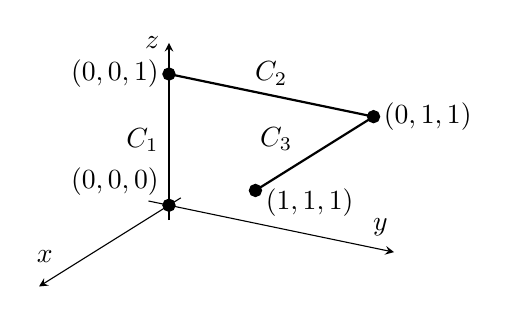
\begin{tikzpicture}[]
\begin{axis}[clip=false,small,view/h=120,axis lines=middle,xlabel={$x$},ylabel={$y$},zlabel={$z$},xtick={\empty},ytick={\empty},ztick={\empty},enlargelimits=true,zlabel style={anchor=east},zmax=1.125]
\addplot3[thick,mark=*]plot coordinates {(0,0,0)(0,0,1)}node[pos=0.5,left]{$C_1$}node[pos=0,above left]{$(0,0,0)$}node[pos=1,left]{$(0,0,1)$};
\addplot3[thick]plot coordinates {(0,0,1)(0,1,1)}node[pos=0.5,above]{$C_2$}node[right]{$(0,1,1)$};
\addplot3[thick,mark=*]plot coordinates {(0,1,1)(1,1,1)}node[pos=0.6,above left]{$C_3$}node[right,yshift=-1ex]{$(1,1,1)$};
\end{axis}
\end{tikzpicture}
\caption{ٹکڑوں میں خطی راہ برائے سوال \حوالہ{سوال_سمتی_تکمل_ٹکڑوں_خطی_راہ}}
\label{شکل_سوال_سمتی_تکمل_ٹکڑوں_خطی_راہ}
\end{minipage}
\end{figure}
\ابتدا{سوال}\شناخت{سوال_سمتی_تکمل_دائری_راہ}
تفاعل \عددی{f(x,y,z)=x+\sqrt{y}-z^2} کا تکمل \عددی{(0,0,0)} تا \عددی{(1,1,1)} درج ذیل راہ پر  چلتے ہوئے  تلاش کریں  (شکل \حوالہ{شکل_سوال_سمتی_تکمل_دائری_راہ})۔
\begin{align*}
C_1:\quad \kvec{r}(t)&=t\ai+t^2\aj,\quad 0\le t\le 1\\
C_2:\quad \kvec{r}(t)&=\ai+\aj+t\ak,\quad 0\le t\le 1
\end{align*}
\انتہا{سوال}
\ابتدا{جواب}
\wf{\unexpanded{\(\tfrac{1}{6}(5\sqrt{5}+9)\)}}
\انتہا{جواب}
%
\ابتدا{سوال}\شناخت{سوال_سمتی_تکمل_ٹکڑوں_خطی_راہ}
تفاعل \عددی{f(x,y,z)=x+\sqrt{y}-z^2} کا تکمل \عددی{(0,0,0)} تا \عددی{(1,1,1)} درج ذیل راہ پر  چلتے ہوئے  تلاش کریں  (شکل \حوالہ{شکل_سوال_سمتی_تکمل_ٹکڑوں_خطی_راہ})۔
\begin{align*}
C_1:\quad \kvec{r}(t)&=t\ak,\quad 0\le t\le 1\\
C_2:\quad \kvec{r}(t)&=t\aj+\ak,\quad 0\le t\le 1\\
C_3:\quad \kvec{r}(t)&=t\ai+\aj+\ak,\quad 0\le t\le 1
\end{align*}

\انتہا{سوال}
%
\ابتدا{سوال}
تفاعل \عددی{f(x,y,z)=\tfrac{x+y+z}{x^2+y^2+z^2}} کا تکمل راہ \عددی{\kvec{r}(t)=t\ai+t\aj+t\ak,\, 0<a\le t\le b} پر تلاش کریں۔
\انتہا{سوال}
\ابتدا{جواب}
\wf{\unexpanded{\(\sqrt{3}\ln\tfrac{b}{a}\)}}
\انتہا{جواب}
%
\ابتدا{سوال}
تفاعل \عددی{f(x,y,z)=-\sqrt{x^2+z^2}} کا تکمل درج ذیل دائری راہ پر تلاش کریں۔
\[\kvec{r}(t)=(a\cos t)\ai+(a\sin t)\ak,\quad 0\le t\le 2\pi\]
\انتہا{سوال}
%
\موٹا{مسطح منحنیات پر لکیری تکملات}\\
سوال \حوالہ{سوال_سمتی_تکمل_دی_گئی_منحنی-الف} تا سوال \حوالہ{سوال_سمتی_تکمل_دی_گئی_منحنی-ب} میں \عددی{f} کا تکمل دی گئی منحنی پر تلاش کریں۔

\ابتدا{سوال}\شناخت{سوال_سمتی_تکمل_دی_گئی_منحنی-الف}
\(f(x,y)=\frac{x^3}{y},\quad C:\, y=\frac{x^2}{2},\quad 0\le x\le 2\)
\انتہا{سوال}
\ابتدا{جواب}
\wf{\unexpanded{\(\tfrac{10\sqrt{5}-2}{3}\)}}
\انتہا{جواب}
%
\ابتدا{سوال}
\(f(x,y)=\frac{x+y^2}{\sqrt{1+x^2}},\quad C:\, y=\frac{x^2}{2},\quad \text{\RL{ \عددی{(1,\frac{1}{2})} سے \عددی{(0,0)} تک}}\)
\انتہا{سوال}
%
\ابتدا{سوال}
\(f(x,y)=x+y,\quad C:\, x^2+y^2=4,\quad \text{\RL{  ربع اول میں \عددی{(2,0)} سے \عددی{(0,2)} تک}}\)
\انتہا{سوال}
\ابتدا{جواب}
\wf{\unexpanded{\(8\)}}
\انتہا{جواب}
%
\ابتدا{سوال}\شناخت{سوال_سمتی_تکمل_دی_گئی_منحنی-ب}
\(f(x,y)=x^2-y,\quad C:\, x^2+y^2=4,\quad \text{\RL{  ربع اول میں \عددی{(0,2)} سے \عددی{(\sqrt{2},\sqrt{2})} تک}}\)
\انتہا{سوال}

\موٹا{کمیت اور معیار اثر}\\
%
\ابتدا{سوال}
ایک پتلی تار جس کی کثافت \عددی{\delta=\tfrac{3}{2}t} ہے منحنی \عددی{\kvec{r}(t)=(t^2-1)\aj+2t\ak,\, 0\le t\le 1} کے ساتھ ساتھ پائی جاتی ہے۔اس تار کی کمیت تلاش کریں۔
\انتہا{سوال}
\ابتدا{جواب}
\wf{\unexpanded{\(2\sqrt{2}-1\)}}
\انتہا{جواب}
%
\ابتدا{سوال}
ایک پتلی  تار جس کی کثافت \عددی{\delta(x,y,z)=15\sqrt{y+2}} ہے منحنی \عددی{\kvec{r}(t)=(t^2-1)\aj+2t\ak,\, -1\le t\le 1} کے ساتھ ساتھ پائی جاتی ہے۔اس تار کا مرکز کمیت تلاش کریں۔ اس منحنی کو ترسیم کر کے اس پر مرکز کمیت دکھائیں۔
\انتہا{سوال}
%
\ابتدا{سوال}
منحنی \عددی{\kvec{r}(t)=\sqrt{2}t\aj+(4-t^2)\ak\, 0\le t\le 1} کے ساتھ ساتھ  ایک پتلی تار پائی جانے والی تار کی کثافت (ا) \عددی{\delta=3t}، (ب) \عددی{\delta=1} ہے۔اس تار کا مرکز کمیت تلاش کریں۔
\انتہا{سوال}
\ابتدا{جواب}
\wf{\unexpanded{
(ا) \عددی{4\sqrt{2}-1}، (ب) \عددی{\sqrt{2}+\ln(1+\sqrt{2})}
}}
\انتہا{جواب}
%
\ابتدا{سوال}
ایک پتلی تار جس کی کثافت \عددی{\delta=3\sqrt{5+t}} ہے منحنی
 \عددی{\kvec{r}(t)=t\ai+2t\aj+\tfrac{2}{3}t^{3/2}\ak,\, 0\le t\le 2} کے ساتھ ساتھ پائی جاتی ہے۔ اس تار کی کمیت تلاش کریں۔
\انتہا{سوال}
%
\ابتدا{سوال}
مستوی \عددی{xy} میں دائرہ \عددی{x^2+y^2=a^2} پر مستقل کثافت \عددی{\delta} کی ایک پتلی تار پائی جاتی ہے۔ محور \عددی{z} کے لحاظ سے اس تار کا جمودی معیار اثر اور رداس  دوار تلاش کریں۔
\انتہا{سوال}
\ابتدا{جواب}
\wf{\unexpanded{
\عددی{I_z=2\pi\delta a^3}، \عددی{R_z=a}
}}
\انتہا{جواب}
%
\ابتدا{سوال}
مستوی \عددی{yz} میں لکیری قطع \عددی{\kvec{r}(t)=t\aj+(2-2t)\ak,\, 0\le t\le 1} پر مستقل کثافت  کی ایک پتلی تار پائی جاتی ہے۔ تینوں محددی محوروں  کے لحاظ سے اس تار کا جمودی معیار اثر اور رداس  دوار تلاش کریں۔
\انتہا{سوال}
%
\ابتدا{سوال}
مستقل کثافت \عددی{\delta} کی ایک پتلی تار پیچدار منحنی \عددی{\kvec{r}(t)=(\cos t)\ai+(\sin t)\aj+t\ak,\, 0\le t\le 2\pi} کے ساتھ ساتھ پائی جاتی ہے۔ (ا) \عددی{I_z} اور \عددی{R_z} تلاش کریں۔ (ب) فرض کریں مستقل کثافت \عددی{\delta} کی ایک دوسری پتلی تار، جس کی لمبائی دگنی ہے (\عددی{0\le t\le 4\pi})، اسی منحنی \عددی{\kvec{r}(t)} کے ساتھ ساتھ پائی جاتی ہے۔ بغیر حل کیے بتلائیں کہ آیا اس تار کا جمودی معیار اثر اور رداس دوار پہلی تار سے مختلف ہوں گے؟  اب انہیں حل کر کے اپنے جواب کی تصدیق کریں۔
\انتہا{سوال}
\ابتدا{جواب}
\wf{\unexpanded{
(ا) \عددی{I_z=2\pi\sqrt{2}\delta}، \عددی{R_z=1}؛\\ (ب) \عددی{I_z=4\pi\sqrt{2}\delta}، \عددی{R_z=1}
}}
\انتہا{جواب}
%
\ابتدا{سوال}
منحنی \عددی{\kvec{r}(t)=(t\cos t)\ai+(t\sin t)\aj+(\tfrac{2\sqrt{2}}{3})t^{3/2}\ak,\, 0\le t\le 1} کے ساتھ ساتھ مستقل کثافت \عددی{\delta =1} کی ایک پتلی تار  پائی جاتی ہے۔ اس کی \عددی{\overline{z}}، \عددی{I_z} اور \عددی{R_z} تلاش کریں۔
\انتہا{سوال}
%
\ابتدا{سوال}
\عددی{I_z} اور \عددی{R_z} مثال \حوالہ{مثال_سمتی_تکمل_قوس_کی_کمیت} کی محراب کے لئے تلاش کریں۔
\انتہا{سوال}
\ابتدا{جواب}
\wf{\unexpanded{
\عددی{I_z=2\pi-2}، \عددی{R_z=1}
}}
\انتہا{جواب}
%
\ابتدا{سوال}
ایک پتلی تار جس کی کثافت \عددی{\delta=\tfrac{1}{t+1}} ہے منحنی \عددی{\kvec{r}(t)=t\ai+\tfrac{2\sqrt{2}}{3}t^{3/2}\aj+\tfrac{t^2}{2}\ak,\, 0\le t\le 2} کے ساتھ ساتھ پائی جاتی ہے۔ اس تار کا مرکز کمیت اور محددی محوروں کے لحاظ سے جمودی معیار اثر اور رداس دوار تلاش کریں۔
\انتہا{سوال}
\موٹا{کمپیوٹر کا استعمال}\\
سوال \حوالہ{سوال_سمتی_تکمل_کمپیوٹر_الف} تا سوال \حوالہ{سوال_سمتی_تکمل_کمپیوٹر_ب} میں کمپیوٹر پر درج ذیل اقدام سے تکمل کی قیمت تلاش کریں۔
\begin{enumerate}[a.]
\item
راہ \عددی{\kvec{r}(t)=g(t)\ai+h(t)\aj+k(t)\ak} کے لئے \عددی{\dif s=\abs{\kvec{v}(t)}\dif t} دریافت کریں۔
\item
متکمل \عددی{f(g(t),h(t),k(t))\abs{\kvec{v}(t)}} کو مقدار معلوم \عددی{t} کا تفاعل لکھیں۔
\item
تکمل \عددی{\int_C f\dif s} کی قیمت مساوات \حوالہ{مساوات_میدان_خطی_تکمل_پ} کی مدد سے حاصل  کریں۔ 
\end{enumerate}
%
\ابتدا{سوال}\شناخت{سوال_سمتی_تکمل_کمپیوٹر_الف}
\(f(x,y,z)=\sqrt{1+30x^2+10y};\quad \kvec{r}(t)=t\ai+t^2\aj+3t^2\ak,\quad 0\le t\le 2\)
\انتہا{سوال}
%
\ابتدا{سوال}
\(f(x,y,z)=\sqrt{1+x^3+5y^3};\quad \kvec{r}(t)=t\ai+\frac{1}{3}t^2\aj+\sqrt{t}\ak,\quad 0\le t\le 2\)
\انتہا{سوال}
%
\ابتدا{سوال}
\(f(x,y,z)=x\sqrt{y}-3z^2;\,\kvec{r}(t)=\cos 2t \ai+\sin 2t\aj+5t\ak,\quad 0\le t\le 2\pi\)
\انتہا{سوال}
%
\ابتدا{سوال}\شناخت{سوال_سمتی_تکمل_کمپیوٹر_ب}
\(f(x,y,z)=\big(1+\frac{9}{4}z^{1/3}\big)^{1/4};\, \kvec{r}(t)=\kvec{r}(t)=\cos 2t \ai+\sin 2t\aj+t^{5/2}\ak,\)\\
\( 0\le t\le 2\pi\quad\quad\quad\quad\quad\quad\)
\انتہا{سوال}
\انتہا{سوالات}
%%%%%%%%%%%%%%%%%%%%%%%%%


